% Emacs settings: -*-mode: latex; TeX-master: "manual.tex"; -*-

\chapter{The \MCX kernel and meta-language}
\label{s:kernel}
\index{Kernel|textbf}

Beamline definitions are written in a special \MCX meta-language which
is translated automatically by the \MCX compiler into a C program
which is in turn compiled to an executable that
performs the simulation. The meta-language is custom-designed for x-ray
scattering and serves two main purposes: (i) to specify the interaction of a
single x-ray with a single optical component, and (ii) to build a
simulation by constructing a complete beamline from individual
components.

For maximum flexibility, efficiency and portability, the meta-language is based on C.
Instrument geometry, propagation of x-rays between the different
components, parameters, data input/output etc. is handled in the
meta-language and by the \MCX compiler. Complex calculations are written in
C embedded in the meta-language description of the
components. However, it is
possible to set up an instrument from existing components and
run a simulation without writing a single line of C code, working
entirely in the meta-language.

Apart from the meta-language, \MCX also includes a number of C library
functions and definitions that are useful for x-ray tracing
simulations. The definitions available for component developers are
listed in appendix~\ref{c:kernelcalls}. The list includes functions
for
\begin{itemize}
\item Computing the intersection between a photon flight-path and various
  objects (such as planes, cylinders, boxes and spheres).
\item Functions for generating random numbers with various distributions.
\item Functions for reading or writing informations from/to data files.
\item Convenient conversion factors between relevant units, etc.
\index{Library!Run-time}
\index{Library!Components!share}
\end{itemize}

The \MCX meta-language was designed to be readable, with a verbose
syntax and explicit mentioning of otherwise implicit information. The
recommended way to get started with the meta-language is to start by
looking at the examples supplied with \MCX, modifying them as necessary
for the application at hand.

\section{Notational conventions}

Simulations generated by \MCX use a semi-classical description of the
x-rays to compute the x-ray trajectory through the instrument and its
interaction with the different components. 

An instrument consists of a list of components through which the x-ray
ray passes one after the other. The order of components is thus significant
since \MCX does not automatically check which component is the next to
interact with the x-ray at a given point in the simulation. Note
that in case of a negative propagation length from one component to the
next, the x-ray is by default \emph{absorbed} as this is often
an indication of unphysical conditions. If a large part of the simulated rays are \emph{absorbed}
on account of this a warning is issued, as this is often caused by a misplaced component.

The instrument is given a global, absolute coordinate system. In
addition, every component in the instrument has its own local coordinate
system that can be given any desired position and orientation (though
the position and orientation must remain fixed for the duration of a
single simulation). \index{Coordinate system}
By convention, the $z$ axis points in the direction of the beam, the $x$ axis
is perpendicular to the beam in the horizontal plane pointing left as seen
from the source, and the $y$ axis points upwards (see \cref{f:axis}).
Nothing in the \MCX metalanguage enforces this convention, but if every component used
different conventions the user would be faced with a severe headache! It is
therefore necessary that this convention is followed by users implementing
new components.
\begin{figure}
  \begin{center}
    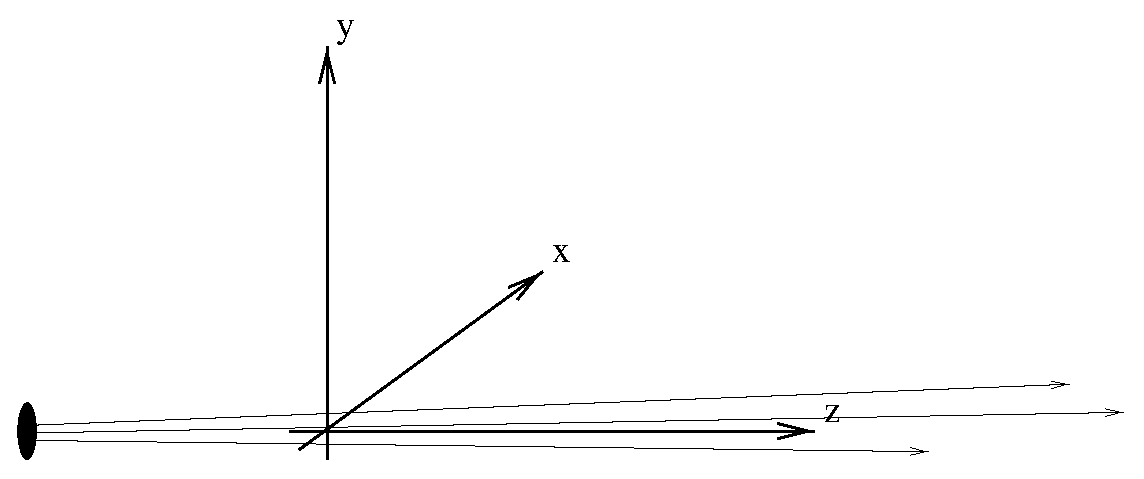
\includegraphics[width=0.8\textwidth]{figures/axis-conventions.eps}
  \end{center}
\caption{conventions for the orientations of the axis in simulations.}
\label{f:axis}
\end{figure}

\index{X-ray state and units}
In the instrument definitions, units of length (\textit{e.g}.\ component
positions) are given in meters and units of angles (\textit{e.g}.\
rotations) are given in degrees.  The state of the x-ray is given by
its position $(x,y,z)$ in \si{m}, its wavevector $(k_x, k_y, k_z)$ in
\si{\per\angstrom}, the time in \si{s},, the phase $\phi$ in \si{\radian}, and a polarisation vector
$\left( E_x, E_y, E_z \right)$, and finally the x-ray weight $p$ in photons~\si{\per s} as described in \cref{c:MCtechniques}.

\section{Syntactical conventions}
\label{s:syntax}

Comments follow the normal C syntax ``\verb+/* ... */+''. C++ style
comments ``\verb+// ...+'' may also be used.
\index{Comments}

%For backward-compatibility
%with early versions, comments may also be written as a percentage sign
%followed by a space (``\verb*+% ...+''), but this is not recommended and
%will be removed in a future version.

Keywords are not case-sensitive, for example ``\verb+DEFINE+'',
``\verb+define+'', and ``\verb+dEfInE+'' are all equivalent. However, by
convention we always write keywords in uppercase to distinguish them
from identifiers and C language keywords. In contrast, \MCX
identifiers (names), like C identifiers and keywords, \emph{are} case
sensitive, another good reason to use a consistent case convention for
keywords. All \MCX keywords are reserved, and thus should not be used
as C variable names. The list of these reserved keywords is shown in table~\ref{t:keywords}. \index{Keyword}

\begin{table}
  \begin{center}
    {\let\my=\\
    \begin{tabular}{|l|c|p{0.7\textwidth}|}
      \hline
      \texttt{Keyword} & Scope & Meaning \\
      \hline
      \texttt{ABSOLUTE} & I & Indicates that the AT and ROTATED keywords are in the absolute coordinate system. \\
      \texttt{AT} & I & Indicates the position of a component in an instrument definition. \\
      \texttt{COPY}& I,C & copy/duplicate an instance or a component definition. \\
      \texttt{DECLARE} & I,C & Declares C internal variables. \\
      \texttt{DEFINE} & I,C & Starts an INSTRUMENT or COMPONENT definition. \\
      \texttt{DEFINITION} & C & Defines component parameters that are constants (\#define). \\
      \texttt{END} & I,C & Ends the instrument or component definition. \\
      \texttt{SPLIT} & I & Enhance incoming statistics by event repetition. \\
      \texttt{EXTEND} & I & Extends a component TRACE section (plug-in). \\
      \texttt{FINALLY} & I,C & Embeds C code to execute when simulation ends. \\
      \texttt{GROUP} & I & Defines an exclusive group of components. \\
      \texttt{\%include} & I,C & Imports an instrument part, a component or a piece of C code (when within embedded C). \\
      \texttt{JUMP} & I & Iterative (loops) and conditional jumps. \\
      \texttt{INITIALIZE} & I,C & Embeds C code to be executed when starting. \\
      \texttt{ITERATE} & I & Defines iteration counter for JUMP. \\
      \texttt{MCDISPLAY} & C & Embeds C code to display component geometry. \\
      \texttt{NEXUS} & I & Defines NeXus output type (4,5,XML,compression). \\
      \texttt{OUTPUT} & C & Defines internal variables to be public and protected symbols (usually all global variables and functions of DECLARE).\\
      \texttt{PARAMETERS} & C & Defines a class of component parameter (DEFINITION, SETTING,STATE). \\
      %\texttt{POLARISATION} & C & Defines neutron polarisation coordinates. \\
      \texttt{PREVIOUS} & C & Refers to a previous component position/orientation.\\
      \texttt{RELATIVE} & I & Indicates that the AT and ROTATED keywords are relative to an other component. \\
      \texttt{ROTATED} & I & Indicates the orientation of a component in an instrument definition. \\
      \texttt{SAVE} & I,C & Embedded C code to execute when saving data. \\
      \texttt{SETTING} & C & Defines component parameters that are
      variables. \\
      \texttt{SHARE} & C & Declares global functions and variables to be shared. \\
      \texttt{STATE} & C & Defines x-ray state coordinates. \\
      \texttt{TRACE} & I,C & Defines the instrument as a the component sequence. \\
      \texttt{WHEN}  & I & Condition for component activation and JUMP.\\
      \hline
    \end{tabular}
    \caption{Reserved \MCX keywords.
    Scope is 'I' for instrument and 'C' for component definitions.}
    \label{t:keywords}
    }
  \end{center}
\end{table}

It is possible, and usual, to split the input instrument definition
across several different files. For example, if a component is not
explicitly defined in the instrument,
\MCX will search for a file containing the component definition in the
standard component library (as well as in the current directory and any
user-specified search directories, see section~\ref{s:files}). It is
also possible to explicitly include another file using a line of the
form \index{Keyword!\%include}
\begin{verbatim}
    %include "file"
\end{verbatim}
Beware of possible confusion with the C language ``\verb+#include+''
statement, especially when it is used in C code embedded within the
\MCX meta-language. Files referenced with ``\verb+%include+'' are read
when the instrument is translated into C by the \MCX compiler, and must
contain valid \MCX meta-language input (and possibly C code). Files referenced with
``\verb+#include+'' are read when the C compiler generates an
executable from the generated C code, and must contain valid C.

Embedded C code is used in several instances in the \MCX
meta-language. Such code is copied by the \MCX compiler into the
generated simulation C program. Embedded C code is written by putting it
between the special symbols \verb|%{| and \verb|%}|, as follows:
\begin{quote}
  \verb|%{| \\
  \hbox to 3em{}\ldots Embedded C code \ldots \\
  \verb|%}|
\end{quote} \index{Embedded C code}
The ``\verb|%{|'' and ``\verb|%}|'' must appear on a line by themselves (do not add comments after).
Additionally, if a ``\verb+%include+'' statement is found \emph{within} an embedded C code block, the specified file will be included from the 'share' directory of the standard component library \index{Library!Components!share} (or from the
current directory and any user-specified search directories) as a C library, just like the usual ``\verb+#include+'' \emph{but only once}. For instance, if many components require
to read data from a file, they may all ask for ``\verb+%include "read_table-lib"+'' \index{Library!read\_table-lib (Read\_Table)} without duplicating the code of this library. If
the file has no extension, both \verb+.h+ and \verb+.c+ files will be searched and included, otherwise, only the specified file will be imported. The \MCX 'run-time' shared
library is included by default (equivalent to ``\verb+%include "mcxtrace-r"+'' in the \texttt{DECLARE} section). \index{Library!Run-time}
For an example of \texttt{\%include}, see the optics/Lens\_simple.comp component. See also section \ref{s:instrdefs-extend} for insertion of full instruments in instruments
  (instrument catenation).

If the instrument description compilation fails, check that the
keywords syntax is correct, that no semi-colon \verb+;+ sign is
missing (e.g. in C blocks and after an ABSORB macro), and there are no name conflicts between instrument and component instances variables.\index{Can not compile}


\section{Writing instrument definitions}
\label{s:instrdefs}
\index{Instruments}

The purpose of the instrument definition file is to specify a sequence of
components, along with their position and parameters, which together
make up a beamline. Each component is given its own local coordinate
system, the position and orientation of which may be specified by its
translation and rotation relative to another component. 
%An example is
%given in section~\ref{s:Samples_vanadium.instr} and some additional
Examples of instrument definitions can be found in the \texttt{example} directory of your 
McXtrace installation. Further examples may be found as they are built on the McXtrace web-page~\cite{mcxtrace_webpage}.

As a summary, the usual grammar for instrument descriptions is
\begin{verbatim}
DEFINE INSTRUMENT name(parameters)
DECLARE C_code
INITIALIZE C_code {NEXUS}
TRACE components
{FINALLY C_code}
END
\end{verbatim}


\subsection{The instrument definition head}

\begin{quote}
  \texttt{DEFINE} \texttt{INSTRUMENT} \textit{name} $(a_1, a_2, \ldots)$
\end{quote} \index{Keyword!DEFINE!INSTRUMENT}
This marks the beginning of the definition. It also gives the name of
the instrument and the list of instrument parameters. Instrument
parameters describe the configuration of the instrument, and usually
correspond to setting parameters of the components, see section \ref{s:compdefs}. A motor position is
a typical example of an instrument parameter. The input parameters of
the instrument constitute the input that the user (or possibly a
front-end program) must supply when the
generated simulation is started.

\index{Parameters!Instruments}
By default, the parameters will be floating point numbers, and will have
the C type \verb+double+ (double precision floating point). The type of
each parameter may optionally be declared to be \verb+int+ for the C
integer type or \verb+char *+ for the C string type. 
%FIXME note on c++ use here
The name \verb+string+ may be used as a synonym for \verb+char *+, and floating
point parameters may be explicitly declared using the name
\verb+double+. The following example illustrates all possibilities:
\begin{quote}
  \texttt{DEFINE INSTRUMENT test(d1, double d2, int i, char *s1, string s2)}
\end{quote}
Here \verb+d1+ and \verb+d2+ will be floating point parameters of C type
\verb+double+, \verb+i+ will be an integer parameter of C type
\verb+int+, and \verb+s1+ and \verb+s2+ will be string parameters of C
type \verb+char *+.
\index{Parameters!Optional, default value}
The parameters of an instrument may be given default values. Parameters with default values are called \emph{optional
  parameters}, and need not be given an explicit value when the
instrument simulation is executed. When executed without any parameter value in the command line (see section~\ref{s:run-sim}), the instrument asks for all parameter values, but pressing the \verb+Return+ key selects the default value (if any). When used with at least one parameter value in the command line, all non specified parameters will have their value set to the default one (if any). A parameter is given a
default value using the syntax ``\textit{param}\texttt{= }\textit{value}''.
For example
\begin{quote}
  \texttt{DEFINE INSTRUMENT test(d1= 1, string s2="hello")}
\end{quote}
Here \verb+d1+ and \verb+d2+ are optional parameters and if no
value are given explicitly, ``1'' and ``hello'' will be used.

Optional parameters can greatly increase the convenience for users of
instruments for which some parameters are seldom changed or of unclear significance to the user. Also, if all instrument parameters have default values, then the simple command \verb+mxdisplay+ \verb+test.instr+ will show the instrument view without requesting any other input, which is usually a good starting point to study the instrument design.

\subsection{The \texttt{DECLARE} section}
\index{Keyword!DECLARE}
\label{s:declare}

\begin{quote}
  \texttt{DECLARE} \\
  \verb|%{| \\
  \hbox to 3em{}\ldots C declarations of global variables etc. \ldots \\
  \verb|%}|
\end{quote} \index{Embedded C code}
This gives C declarations that may be referred to in the rest of the
instrument definition. A typical use is to declare global variables or
small functions that are used elsewhere in the instrument. The \verb+%include ''file''+ keyword may be used to import a specific
component definition or a part of an instrument. Variables defined here are global, and may conflict with internal \MCX variables, particularly symbols like
\verb+x,y,z,Ex,Ey,Ez,kx,ky,kz,t,phi+ and generally all names starting with \verb+mc+ nad \verb+mx+ should be avoided. If you can not compile the instrument, this may be the reason.
\index{Can not compile}The \texttt{DECLARE} section is optional.

\subsection{The \texttt{INITIALIZE} section}
\index{Keyword!INITIALIZE}
\label{s:initialize}

\begin{quote}
  \texttt{INITIALIZE} \\
  \verb|%{| \\
  \hbox to 3em{}\ldots C initializations. \ldots \\
  \verb|%}|
\end{quote} \index{Embedded C code}
This section contains code that is executed once when the simulation starts. This section is
optional. Instrument setting parameters may be modified in this section (e.g. doing tests or automatic settings).

\subsection{The \texttt{NEXUS} extension}
\index{Keyword!NEXUS} \index{Tools!NeXus} \index{Tools!HDF} \index{Data formats}
\label{s:nexus}

To use the NeXus format~\cite{nexus_webpage} the simulation must be linked with additional libraries (HDF and NeXus) which must have been pre-installed. Preferrably, \MCX should
have been installed with the \verb+./configure --with-nexus+ on Unix/Linux systems. To activate the NeXus output, the instrument must be compiled with the flags
\verb+-DUSE_NEXUS -lNeXus+.

The default NeXus format is NeXus 5 with compression. However, that format may be changed with the optional keyword \verb+NEXUS+ to follow the INITIALIZE section, namely:

\begin{quote}
  \texttt{INITIALIZE} \\
  \verb|%{| \\
  \hbox to 3em{}\ldots C initializations. \ldots \\
  \verb|%}|
  \verb+NEXUS {"4"|"5"|"XML"|"compress"|"zip"}+
\end{quote}

It is possible to set the type of NeXus file with a string argument, containing words "4", "5" or "XML". Optionally, if the string also contains the \verb+compress+ or \verb+zip+
word, the NeXus file will use compression for Data Sets. We recommend the syntax \verb+NEXUS "5 compress"+ which is the default.

You may choose the name of the output file with the \verb+-f filename+ option from the instrument executable or \verb+mxrun+ (see Sections \ref{s:run-sim}, \ref{s:mxrun} and Table
\ref{f:simoptions2}).

Then, the output format is chosen as usual with the \verb+--format=NeXus+ option when launching the simulation. All output files are stored in the output \textit{filename}, as well
as the instrument description itself. Other formats are still available. When run on a distributed system (e.g. MPI), detectors are gathered, but list of events (see e.g. component
Virtual\_output) are stored as one data set per node.

\subsection{The \texttt{TRACE} section}
\index{Keyword!TRACE}
\label{s:trace}


As a summary, the usual grammar for component instances within the instrument TRACE section is
\begin{verbatim}
COMPONENT name = comp(parameters)
  AT (...) [RELATIVE [reference|PREVIOUS] | ABSOLUTE]
 {ROTATED  {RELATIVE [reference|PREVIOUS] | ABSOLUTE} }
\end{verbatim}

The \texttt{TRACE} keyword starts a section giving the list of
components that constitute the instrument.
Components are declared like this:
\begin{quote}
  \texttt{COMPONENT} $\textit{name} =
    \textit{comp}(p_1 = e_1, p_2 = e_2, \ldots)$
\end{quote}
\index{Components}
\index{Keyword!COMPONENT} \index{Parameters!Setting}
\index{Parameters!Definition}
This declares a component named \textit{name} that is an instance of the
component definition named \textit{comp}. The parameter list gives the
setting and definition parameters for the component. The expressions $e_1,
e_2, \ldots$ define the values of the parameters. For setting parameters
arbitrary ANSI-C expressions may be used, while for definition parameters
only \emph{constant} numbers, strings, names of instrument parameters, or names
of C identifiers are allowed (see section~\ref{s:comp-header} for details of
the difference between definition and setting parameters). To assign the
value of a general expression to a definition parameter, it is necessary to
declare a variable in the \texttt{DECLARE} section, assign the value to the
variable in the \texttt{INITIALIZE} section, and use the variable as the
value for the parameter.

The \MCX program takes care to rename parameters appropriately in the
output so that no conflicts occur between different component
definitions or between component and instrument definitions. It is thus
possible (and common) to use a component definition multiple times
in an instrument description.

Be aware of the C variable type conversions when setting numerical parameter values, as in \verb+p1=12/1000+. In this example, the parameter \verb+p1+ will be set to 0 as the division of
the two integers is indeed 0. To avoid that, use explicitely floating type numbers as in \verb+p1=12.0/1000+.\index{Bugs}

The \MCX compiler will automatically search for a file containing a
definition of the component if it has not been declared previously. The
definition is searched for in a file called ``\textit{name\/}\texttt{.comp}''. See
section~\ref{s:files} for details on which directories are searched. This
facility is often used to refer to existing component definitions in
standard component libraries. It is also possible to write component
definitions in the main file before the instrument definitions, or to
explicitly read definitions from other files using \verb+%include+
(not within embedded C blocks).

The physical position of a component is specified using an \texttt{AT} modifier
following the component declaration:
\index{Keyword!AT} \index{Keyword!RELATIVE} \index{Keyword!ABSOLUTE}
\begin{quote}
  \texttt{AT} $(x,y,z)$ \texttt{RELATIVE} \textit{name}
\end{quote}
This places the component at position $(x,y,z)$ in the coordinate system
of the previously declared component \textit{name}. Placement may also
be absolute (not relative to any component) by writing
\begin{quote}
  \texttt{AT} $(x,y,z)$ \texttt{ABSOLUTE}
\end{quote}
Any C expression may be used for $x$, $y$, and $z$. The \texttt{AT}
modifier is required.
Rotation is achieved similarly by writing \index{Keyword!ROTATED}
\begin{quote}
  \texttt{ROTATED} $(\phi_x,\phi_y,\phi_z)$ \texttt{RELATIVE} \textit{name}
\end{quote}
This will result in a coordinate system that is rotated first the angle $\phi_x$ (in degrees) around the $x$ axis, then $\phi_y$ around the $y$ axis, and finally
$\phi_z$ around the $z$ axis. Rotation may also be specified using \texttt{ABSOLUTE} rather than \texttt{RELATIVE}. If no rotation is
specified, the default is $(0,0,0)$ using the same relative or absolute specification used in the \texttt{AT} modifier. We recommend to apply all rotations of an instrument
description on Arm class components only, acting as goniometers, and position the optics on top of these. This usually makes it much easier to orient pieces of the beamline, and
avoid positioning errors.

The \emph{position} of a component is actually the origin of its local coordinate system. Usually, this is used as the input window position (e.g. for guide-like components), or
the center position for cylindrical/spherical components.

The \texttt{PREVIOUS} \index{Keyword!PREVIOUS} keyword is a generic name to refer to the previous component in the simulation. Moreover, the \texttt{PREVIOUS(n)} keyword will refer
to the $n$-th previous component, starting from the current component, so that \texttt{PREVIOUS} is equivalent to \texttt{PREVIOUS(1)}. This keyword should be used after the
\texttt{RELATIVE} keyword, but not for the first component instance of the instrument description.
\begin{quote}
  \texttt{AT} $(x,y,z)$ \texttt{RELATIVE} \texttt{PREVIOUS}
  \texttt{ROTATED} $(\phi_x,\phi_y,\phi_z)$ \texttt{RELATIVE} \texttt{PREVIOUS(2)}
\end{quote}
Invalid \texttt{PREVIOUS} references will be assumed to be absolute placement.

The order and position of components in the \texttt{TRACE} section does not
allow components to overlap, except for particular cases (see the \texttt{GROUP} keyword below).
Indeed, many components of the \MCX library \index{Library!Components} start
by propagating the x-ray event to the begining of the component itself.
If the corresponding propagation length is found to be negative
(\textit{i.e.} the x-ray is already \emph{after} or \emph{aside} the component, and has thus
passed the 'active' position), the x-ray event is ABSORBed, resulting in a zero intensity and event counts after a given position. The number of such removed x-rays is indicated at the end of the simulation.
Getting such warning messages may be an indication that either some
components overlap, or some x-rays are getting outside of the
simulation, for instance this usually happens after a monochromator,
as the non-reflected beam is indeed lost. A special warning appears
when no x-ray has reached some part of the simulation. This is usually the sign of either overlapping components or a very low intensity. \index{Removed x-ray events}

For experienced users, we recommend as well the usage of the \texttt{WHEN} and \texttt{EXTEND} keywords, as well as other syntax extensions presented in section \ref{s:instrdefs-extend} below.

\subsection{The \texttt{SAVE} section}
\index{Keyword!SAVE}
\label{s:save}

\begin{quote}
  \texttt{SAVE} \\
  \verb|%{| \\
  \hbox to 3em{}\ldots C code to execute each time a temporary save is required \ldots \\
  \verb|%}|
\end{quote} \index{Signal handler!USR2 signal}
This gives code that will be executed when the simulation is requested to save data, for instance when receiving a USR2 signal (on Unix systems), or using the \verb+Progress_bar+ component with intermediate savings. It is also executed when the simulation ends. This section is optional.

\subsection{The \texttt{FINALLY} section}
\index{Keyword!FINALLY}
\label{s:finally}

\begin{quote}
  \texttt{FINALLY} \\
  \verb|%{| \\
  \hbox to 3em{}\ldots C code to execute at end of simulation \ldots \\
  \verb|%}|
\end{quote}
This gives code that will be executed when the simulation has
ended. When existing, the \texttt{SAVE} section is first executed. The
\texttt{FINALLY} section is optional.
A simulation may be requested to end before all x-rays have been
traced when recieving a TERM or INT signal (on Unix systems), or with
Control-C, causing code in \texttt{FINALLY} to be evaluated.
\index{Signal handler!TERM signal} \index{Signal handler!INT signal}


\subsection{The end of the instrument definition}
\label{s:end}
\index{Keyword!END}

The end of the instrument definition must be explicitly marked using the keyword
\begin{quote}
  \texttt{END}
\end{quote}

%\subsection{Code for the instrument \texttt{vanadium\_example.instr}}
%\label{s:Samples_vanadium.instr}
%A commented instrument definition taken from the \texttt{examples} directory is
%here shown as an example of the use of \MCX .
%FIXME \smallverbatimfile{../../McCode/trunk/nlib/examples/Samples_vanadium.instr}



\section{Writing instrument definitions - complex arrangements and syntax}
\label{s:instrdefs-extend}
\index{Instruments}

In this section, we describe some additional ways to build instruments using groups, code extension, conditions, loops and duplication of components.

As a summary, the nearly complete grammar definition for component instances within the instrument TRACE section is:

\begin{verbatim}
{SPLIT} COMPONENT name = comp(parameters) {WHEN condition}
  AT (...) [RELATIVE [reference|PREVIOUS] | ABSOLUTE]
  {ROTATED {RELATIVE [reference|PREVIOUS] | ABSOLUTE} }
  {GROUP group_name}
  {EXTEND C_code}
  {JUMP [reference|PREVIOUS|MYSELF|NEXT] [ITERATE number_of_times | WHEN condition] }
\end{verbatim}

\subsection{Embedding instruments in instruments TRACE}
\index{Keyword!\%include}
\label{s:instrdefs-include-instr}
The \texttt{\%include} insertion mechanism may be used within the TRACE section, in order to concatenate instruments. This way, each DECLARE, INITIALIZE, SAVE, and FINALLY C
 blocks, as well as instrument parameters from each part are catenated. The TRACE section is made of inserted COMPONENTS from each part. In principle, it then possible to write an
 instrument as:
\begin{verbatim}
DEFINE catenated()
TRACE

%include "part1.instr"
%include "part2.instr"

END
\end{verbatim}
where each inserted instrument is a valid full instrument. In order to avoid some components to be duplicated - e.g. Sources from each part - a special syntax in the TRACE section
\begin{verbatim}
INSTRUMENT COMPONENT a=...
\end{verbatim}
marks the component \textit{a} as removable when inserted. In principle, inserted instruments may themselves use \texttt{\%include}.

\subsection{Component extensions - EXTEND}
\index{Keyword!EXTEND}
\label{s:instrdefs-extend}

It is sometimes desirable to slightly modify an existing component of the \MCX library. One would usually make a copy of the component, and extend the code of its \texttt{TRACE}
section. \MCX provides an easy way to change the behaviour of existing components in an instrument definition without duplicating files, using the \texttt{EXTEND} modifier
\index{Keyword!EXTEND}
\begin{quote}
  \texttt{EXTEND} \\
  \verb|%{| \\
  \hbox to 3em{}\ldots C code executed after the component TRACE section \ldots \\
  \verb|%}|
\end{quote} \index{Embedded C code}
The embedded C code is appended to the component \texttt{TRACE} section, and all its internal variables (as well as all the \texttt{DECLARE} instrument variables, \emph{except} instrument parameters) may be used. To use instrument parameters, you should copy them into global variables in the DECLARE instrument section, and refer to these latter.
This component declaration modifier is of course optional. You will find usage examples in the Component manual\cite{mcxtrace-comp-manual}.

\subsection{Mutually exclusive components in parallell - GROUP} 
\index{Keyword!GROUP}
\label{s:instrdefs-group}
In some configurations it is necessary to position one or
more groups of components, nested, in parallel, or overlapping. One
example is a multiple crystal monochromator. One would then like the
x-ray to interact with \emph{one of} the components of the group
and then continue.

In order to handle such arrangements without removing x-rays, groups are defined by the \texttt{GROUP} modifier (after the AT-ROTATED positioning):
\begin{quote}
  \texttt{GROUP} \textit{name}
\end{quote}
to all involved component declarations. \index{Keyword!GROUP}
All components of the same named group are tested one after the other,
until one of them interacts (uses the SCATTER
macro\index{Library!Run-time!SCATTER}). The selected component acts on
the x-ray, and the rest of the group is skipped. Such groups are thus exclusive (only one of the elements is active).

Within a \texttt{GROUP}, \emph{all} \texttt{EXTEND} sections of the group are executed. In order to discriminate components that are active from those that are skipped, one may use the SCATTERED flag, which is set to zero when entering each component or group, and incremented when the x-ray is SCATTERed, as in the following example \index{Library!Run-time!SCATTER} \index{Library!Run-time!SCATTERED}
\begin{quote}
  \texttt{COMPONENT} $\textit{name0} =
    \textit{comp}(p_1 = e_1, p_2 = e_2, \ldots)$ \\
    \hbox to 1em{} \texttt{AT} $(0,0,0)$ \texttt{ABSOLUTE} \\
  \texttt{COMPONENT} $\textit{name1} =
    \textit{comp}(\ldots)$ \texttt{AT} $(...)$  \texttt{ROTATED} $(...)$ \\
  \hbox to 1em{} \texttt{GROUP} \textit{GroupName} \texttt{EXTEND} \\
  \hbox to 1em{} \verb|%{| \\
  \hbox to 3em{} \verb+if (SCATTERED) printf("I scatter");+\\
  \hbox to 3em{} \verb+else printf("I do not scatter");+\\
  \hbox to 1em{} \verb|%}| \\
  \texttt{COMPONENT} $\textit{name2} =
    \textit{comp}(\ldots)$ \texttt{AT} $(...)$ \texttt{ROTATED} $(...)$ \\
  \hbox to 1em{} \texttt{GROUP} \textit{GroupName}
\end{quote}
Components \emph{name1} and \emph{name2} are at the same position. If the first one intercepts the x-ray (and has a SCATTER within its \texttt{TRACE} section), the SCATTERED variable becomes true, the code extension will result in printing "I scatter", and the second component will be skipped.
Thus, we recommend to make use of the SCATTER keyword each time a component 'uses' the x-ray (scatters, detects, \ldots) within component definitions (see section \ref{s:compdefs}). Also, the components to be grouped should be consecutive in the TRACE section of the instrument, and the GROUPed section should not contain components which are not part of the group.

Note that a \texttt{GROUP} construct is \emph{not} applicable to a situation where an x-ray which has interacted (\texttt{SCATTER}ed) with one component in the group, may interact
with another. In this case a more complex arrangement is needed. See \cite{willendrup2011using} for a description of how to do this in \MCS. This is approach is \emph{directly} applicable in \MCX without modification. 

Combining EXTEND, GROUP and WHEN can result in unexpected behaviour. Please read the related warning at the end of section \ref{s:instrdefs-extend-when}.

\subsection{Duplication of component instances - COPY}
\index{Keyword!COPY}
\label{s:instrdefs-extend-copy}

Often, one has a set of similar component instances in an instrument. These could be e.g. a set of identical monochromator blades, or a set of detectors.
Together with JUMPs (see below), there is a way to copy a component instance, duplicating a parameter set, as well as any EXTEND, GROUP, JUMP and WHEN keyword.
Position (AT) and rotation (ROTATED) specification must be explicitely entered in order to avoid component overlap.

The syntax for instance copy is
\begin{quote}
  \texttt{COMPONENT} name = \texttt{COPY}(instance\_name)
\end{quote}
where \textit{instance\_name} is the name of a preceeding component instance in the instrument. It may be 'PREVIOUS' as well.

If you would like to change only some of the parameters in the instance copy, you may write, e.g.:
\begin{quote}
  \texttt{COMPONENT} name = \texttt{COPY}(instance\_name)(par1=0, par2=1)
\end{quote}
which will override the original instance parameter values. In case EXTEND, GROUP, JUMP and WHEN
keywords are defined for the copied instance, these will override the settings
from the copied instance.

In the case where there are many duplicated components all originating from the same instance, there is a mechanism for automating copied instance names:
\begin{quote}
  \texttt{COMPONENT} \texttt{COPY}(root\_name) = \texttt{COPY}(instance\_name)
\end{quote}
will append a unique number to \textit{root\_name}, to avoid name
conflicts. As a side effect, referring to this component instance (for
e.g. further positioning) is not straight forward as the name is
determined by \MCX and does not depend completely on the user's
choice, even though the PREVIOUS keyword may still be used. We thus recommend to use this naming mechanism only for components which should not be refered to in the instrument.

This automatic naming may be used anywhere in the TRACE section of the instrument, so that all components which do not need further referral may be labeled as COPY(Origin).

As an example, we show how to have a set of three equivalent pinholes (Slits). Only the first instance of the Slit component is defined explicitly, whereas following instances are
copies of that definition. The instance names of \texttt{Slit} components are set automatically.

\begin{verbatim}
COMPONENT S_in = Arm() AT (...)

COMPONENT S_1  = Slit(radius=0.1)
  AT (0,0,0) RELATIVE PREVIOUS

COMPONENT COPY(S_1)  = COPY(S_1)
  AT (0,0,d) RELATIVE PREVIOUS

COMPONENT COPY(S_1)  = COPY(S_1)
  AT (0,0,d) RELATIVE PREVIOUS
...
COMPONENT S_Out = Arm() AT (0,0,d) RELATIVE PREVIOUS
\end{verbatim}

\subsection{Conditional components - WHEN}
\index{Keyword!WHEN}
\label{s:instrdefs-extend-when}

One of the most useful features of the extended \MCX syntax is the conditional \texttt{WHEN} modifier. This optional keyword comes before the AT-ROTATED positioning. It basically
enables the component only when a given condition is true (non null).

\begin{quote}
  \texttt{COMPONENT} $\textit{name} = \textit{comp}(p_1 = e_1, p_2 = e_2, \ldots)$
  \texttt{WHEN} (\textit{condition})
\end{quote}
The condition has the same scope as the EXTEND modifier, i.e. may use component internal variables as well as all the \texttt{DECLARE} instrument variables.

Usage examples could be to have specific monitors only sensitive to selected processes, or to have components which are only present under given circumstances (e.g. removable
filter or radial collimator), or to select a sample among a set of choices.

In the following example, an EXTEND block sets a condition when a scattering event is encoutered, and the following monitor is then activated.
\begin{verbatim}
COMPONENT Sample = V_sample(...) AT ...
  EXTEND
  %{
    if (SCATTERED) flag=1; else flag=0;
  %}

COMPONENT MyMon = Monitor(...) WHEN (flag==1)
  AT ...
\end{verbatim}

The WHEN keyword only applies to the TRACE section and related EXTEND blocks of instruments/components. Other sections (INITIALIZE, SAVE, MCDISPLAY, FINALLY) are executed
independently of the condition. As a side effect, the 3D view of the instrument (\texttt{mxdisplay}) will show all components as if all conditions were true.

A usage example of the WHEN keyword can be found in the \\
\verb+X-ray site/ESRF/ESRF_ID11+ instrument from the \verb+mxgui+, where the source model may be chosen by an external parameter.

The \texttt{WHEN} keyword is compatible with \texttt{GROUP}, and thus may be used to activate/deactivate members in a \texttt{GROUP} just like non-grouped components. 
Combining \texttt{WHEN}, \texttt{EXTEND} and \texttt{GROUP} can result in unexpected behaviour, please use them with caution! As an example, let a \texttt{GROUP} of components all
have the same \texttt{WHEN} condition.
If the condition is false, none of the elements \texttt{SCATTER}, meaning that all x-rays will be \texttt{ABSORB}ed. As a solution to this problem, we propose to include an
\texttt{EXTEND}ed Arm
component in the \texttt{GROUP}, but with the opposite \texttt{WHEN} condition and a \texttt{SCATTER} keyword in the \texttt{EXTEND} section. This means that when none of the other
\texttt{GROUP} elements are present, the Arm
will be present and \texttt{SCATTER}.


\subsection{Component loops and non sequential propagation - JUMP}
\index{Keyword!JUMP}
\index{Keyword!ITERATE}
\index{Keyword!WHEN}
\label{s:instrdefs-extend-jump}

There are situations in which one would like to repeat a given component many times, or under a given condition. The JUMP modifier is meant for that and should be mentioned after
the positioning, GROUP and EXTEND. This breaks the sequential propagation along components in the instrument description. There may be more than one JUMP per component instance.

The jump may depend on a condition:
\begin{quote}
  \texttt{COMPONENT} $\textit{name} = \textit{comp}(p_1 = e_1, p_2 = e_2, \ldots)$
  \texttt{AT} (...)
  \texttt{JUMP} \textit{reference} WHEN \textit{condition}
\end{quote}
in which case the instrument TRACE will jump to the \textit{reference} when \textit{condition} is true.

The \textit{reference} may be an instance name, as well as PREVIOUS, PREVIOUS($n$), MYSELF, NEXT, and NEXT($n$), where $n$ is the index gap to the target either backward (PREVIOUS) or forward (NEXT), so that PREVIOUS(1) is PREVIOUS and NEXT(1) is NEXT. MYSELF means that the component will be iterated as long as the condition is true. This may be a way to handle multiple scattering, if the component has been designed for that.

The jump arrives directly inside the target component, in the local coordinate system (i.e. without applying the AT and ROTATED keywords). In order to better control the target
positions, it is \emph{required} that, except for looping MYSELF, the target component type should be an \emph{Arm}.
%
%There is a more general way to iterate components, which consists in repeating the loop for a given number of times.
%\begin{quote}
%  \texttt{JUMP} \textit{reference} ITERATE \textit{number\_of\_times}
%\end{quote}
%This method is specially suited for very long curved guides of similar components, but in order to take into account rotation and translation between guide sections, the iterations are performed between Arm's.
%
%In the following example for a curved guide made on $n=500$ elements of length $L$ on a curvature radius $R$, with gaps $d$ between elements, we simply write:
%\begin{verbatim}
%COMPONENT CG_In = Arm() AT (...)
%
%COMPONENT CG_1  = Guide_gravity(l=L/n, m=1, ...)
%  AT (0,0,0) RELATIVE PREVIOUS
%
%COMPONENT CG_2_Position = Arm()
%  AT (0,0,L/n+d) RELATIVE PREVIOUS
%  ROTATED (0, (L/n+d)/R*180/PI, 0) RELATIVE PREVIOUS
%
%COMPONENT CG_2  = Guide_gravity(l=L/n, m=1, ...)
%  AT (0,0,0) RELATIVE PREVIOUS
%  ROTATED (0, (L/n+d)/R*180/PI, 0) RELATIVE PREVIOUS
%  JUMP CG_2_Position ITERATE n
%...
%COMPONENT CG_Out = Arm() AT (0,0,L/n) RELATIVE PREVIOUS
%\end{verbatim}
%
Similarly to the \texttt{WHEN} modifier (see section \ref{s:instrdefs-extend-when}), \texttt{JUMP} only applies within the TRACE section of the instrument definition. Other
sections (INITIALIZE, SAVE, MCDISPLAY, FINALLY) are exectuted independently of the jump. As a side effect, the 3D view of the instrument \texttt{mxdisplay} will show components as if
there was no jump. This means that in the following example, the very long mirror 3D view only shows a single mirror element.

It is \emph{not} recommended to use the \verb+JUMP+ inside \verb+GROUP+s, as the JUMP condition/counter applies to the component instance within its group.

We would like to emphasize the potential errors originating from such
jumps. Indeed, imbricating many jumps may lead to situations were it
is difficult to understand the flow of the simulation. We thus recommend the usage of JUMPs only for experienced and cautious users.\index{Bugs}

\subsection{Enhancing statistics reaching components - SPLIT}
\index{Keyword!SPLIT}
\label{s:instrdefs-extend-enhance}

The following method applies when the incoming x-ray event distribution is considered to be representative of the real beam, but x-rays are lost in the course of propagation (with
low efficiency processes, absorption, etc). Then, one may think that it's a pity to have so few events reaching the 'interesting' part of the beamline (usually close to the end
of the instrument description).
If some components make extensive use of random numbers (MC choices), they shuffle this way the distributions, so that identical incoming events will not produce the same outgoing
event. In this case, you may want to use a technique known as \emph{stratified sampling} (see \cref{c:MCtechniques}) which in \MCX is implemented through the \verb+SPLIT+ keyword with the syntax

\begin{quote}
  \texttt{SPLIT} ${r}$ \texttt{COMPONENT} $\textit{name} = \textit{comp}(\ldots)$
\end{quote}

where the optional number $r$ specifies the number of repetitions for each event. Default is $r=10$.
Each x-ray event reaching component \textit{name} will be repeated $r$ times with a weight divided by $r$, so that in practice the number of events for the remaining part of the
simulation (down to the END), will potentially have more statistics. This is only true if following components (and preferably component \textit{name}) use random numbers. You may
use this method as many times as you wish in the same instrument, e.g. at the monochromator and sample position. This keyword can also be used within a GROUP. The efficiency is
roughly $r$ raised to the number of occurences in the instrument, so that enhancing two components with the default $r=10$ will produce an enhancement effect of $100$ wrt.
the number of events at the end. The execution time will increase but at a slower rate than the statistical quality, provided that the above criteria are met. If the
instrument makes use of global variables - e.g. in conjunction with a WHEN or User Variable monitoring (see Monitor\_nD) - you should take care that these variables are set
properly for each SPLIT loop, which usually means that they must be reset inside the SPLITed section and assigned/used further on. \index{Bugs}


%A usage example of the SPLIT keyword can be found in the \\
%\verb+X-ray site/ILL/ILL_H15_IN6+ instrument from the \verb+mcgui+, to enhance statistics for x-rays scattering on monochromators and sample.

\section{Writing component definitions}
\label{s:compdefs}

The purpose of a \MCX component is to model the interaction of an
x-ray with a physical component of a real beamline. Given the
state of the incoming x-ray, the
component definition calculates the state of the x-ray when it leaves
the component.  The calculation of the effect of the component on the
x-ray is performed by a block of embedded C code.
One example of a component definition is given in \cref{s:slit}, and all
component definitions can be found on the \MCX
web-page~\cite{mcxtrace_webpage} and described in the \MCX component manual.

A large number of functions and constants are available in
order to write efficient components. See \cref{c:kernelcalls}
for
\begin{itemize}
\item x-ray propagation functions
\item geometric intersection time computations
\item mathematical functions
\item random number generation
\item physical constants
\item coordinate retrieval and operations
\item file generation routines (for monitors),
\item data file reading
\end{itemize}

%A component definition looks as follows:


\subsection{The component definition header}
\label{s:comp-header}

\begin{quote}
  \texttt{DEFINE} \texttt{COMPONENT} \textit{name}
\end{quote}
\index{Keyword!DEFINE!COMPONENT}
This marks the beginning of the definition, and defines the name of the
component.
\begin{quote}
  \texttt{DEFINITION} \texttt{PARAMETERS} $(d_1, d_2, \ldots)$ \\
  \texttt{SETTING} \texttt{PARAMETERS} $(s_1, s_2, \ldots)$
\end{quote}
\index{Keyword!DEFINITION PARAMETERS}
\index{Keyword!SETTING PARAMETERS}
This declares the definition and setting parameters of the component.
These parameters can be
accessed from all sections of the component (see below),
as well as in \verb+EXTEND+ sections of the instrument definition (see section~\ref{s:instrdefs}).
\index{Parameters!Setting}
\index{Parameters!Definition}

Setting parameters are translated into C variables usually of type
\verb+double+ in the generated simulation program, so they are usually
numbers. Definition parameters are translated into \verb+#define+ macro
definitions, and so can have any type, including strings, arrays, and
function pointers.

However, because of the use of \verb+#define+, definition parameters
suffer from the usual problems with C macro definitions. Also, it is not
possible to use a general C expression for the value of a definition
parameter in the instrument definition, only constants and variable
names may be used. For this reason, setting parameters should be used
whenever possible.

Outside the \verb+INITIALIZE+ section of components, changing setting parameter values only affects the current section.

There are a few cases where the use of definition parameters instead of
setting parameters makes sense. If the parameter is not numeric, nor a character string ({\em i.e.} an
array, for example), a setting parameter cannot be
used. Also, because of the use of \verb+#define+, the C compiler can
treat definition parameters as constants when the simulation is
compiled. For example, if the array sizes of a multidetector are
definition parameters, the arrays can be statically allocated in the
component \verb+DECLARE+ section. If setting parameters were used, it
would be necessary to allocate the arrays dynamically using {\em e.g.}\
\verb+malloc()+.

Setting parameters may optionally be declared to be of type
\verb+int+, \verb+char *+ and \verb+string+, just as in the instrument definition (see section~\ref{s:instrdefs}).

\begin{quote}
  \texttt{OUTPUT} \texttt{PARAMETERS} $(s_1, s_2, \ldots)$
\end{quote}
\index{Keyword!OUTPUT PARAMETERS}
\index{Parameters!Protecting|see{Keyword/OUTPUT}}
This declares a list of C identifiers (variables, functions) that are
output parameters (\textit{i.e.} global) for the
component. Output parameters are used to hold values that are computed
by the component itself, rather than being passed as input. This could
for example be a count of x-rays in a detector or a constant that is
precomputed to speed up computation.

Using \texttt{OUTPUT PARAMETERS} is \emph{highly} recommended for
\texttt{DECLARE} and internal/global component variables and functions
in order to prevent that instances of the same component use the same variable names. Moreover (see section \ref{s:comp-declare} below), these may be accessed from any other instrument part (e.g. using the \verb+MC_GETPAR+ C macro).
On the other hand, the variables from the SHARE sections should \emph{not}
be defined as OUTPUT parameters.

The \texttt{OUTPUT} \texttt{PARAMETERS} section is optional.

\subsubsection{Optional component parameters}
\index{Parameters!Optional, default value}

Just as for instrument parameters, the definition and setting parameters of a
component may be given a default value. Parameters with default values are
called \emph{optional parameters}, and need not be given an explicit value when
the component is used in an instrument definition. A parameter is given a
default value using the syntax ``\textit{param}\texttt{ = }\textit{value}''.
For example
\begin{quote}
  \texttt{SETTING PARAMETERS (radius, height, pack= 1)}
\end{quote}
Here \verb+pack+ is an optional parameter and if no value is given
explicitly, ``1'' will be used. In contrast, if no value is
  given for \texttt{radius} or \texttt{height}, an error message will
  result.

Optional parameters can greatly increase the convenience for users of
components with many parameters that have natural default values which
are seldom changed. Optional parameters are also useful to preserve
backwards compatibility with old instrument definitions when a component
is updated. New parameters can be added with default values that
correspond to the old behavior, and existing instrument definitions can
be used with the new component without changes.

Optional parameters should not be used in cases where no
natural default value exists. For example the size of a slit should not be given a default value. 
This would prevent the error messages that should be given in the common case of a
user forgetting to set an important parameter.


\subsection{The \texttt{DECLARE} section}
\label{s:comp-declare}
\begin{quote}
  \texttt{DECLARE} \\
  \verb|%{| \\
  \hbox to 3em{}\ldots C code declarations (variables, definitions, functions)\ldots \\
  \hbox to 3em{}\ldots These are usually OUTPUT parameters to avoid name conflicts \ldots \\
  \verb|%}|
\end{quote}
\index{Keyword!DECLARE}
This gives C declarations of global variables, functions, etc. that are used by the
component code. This may for instance be used to declare a x-ray
counter for a detector component. This section is optional.

Note that any variables declared in a \verb+DECLARE+ section are
\emph{global}. Thus a name conflict may occur if two instances of a
component are used in the same instrument. To avoid this, variables
declared in the \texttt{DECLARE} section should be \texttt{OUTPUT} parameters of
the component because \MCX will then rename variables to avoid conflicts.
For example, a simple detector might be defined as follows:
\begin{quote}
\begin{verbatim}
DEFINE COMPONENT Detector
OUTPUT PARAMETERS (counts)
DECLARE
%{
  int counts;
%}
...
\end{verbatim}
\end{quote}
\index{Keyword!OUTPUT PARAMETERS}
\index{Library!Run-time!MC\_GETPAR}
The idea is that the \texttt{counts} variable counts the number of
x-rays detected. In the instrument definition, the \texttt{counts}
parameter may be referenced using the \verb+MC_GETPAR+ C macro, as in
the following example instrument fragment:\label{mcgetpar}
\begin{quote}
\begin{verbatim}
COMPONENT d1 = Detector()
...
COMPONENT d2 = Detector()
...
FINALLY
%{
  printf("Detector counts: d1 = %d, d2 = %d\n",
         MC_GETPAR(d1,counts), MC_GETPAR(d2,counts));
%}
\end{verbatim}
\end{quote}
This way, \MCX takes care to transparently rename the two 'counts'
\texttt{OUTPUT} parameters so that they are distinct, and can be
accessed from elsewhere in the instrument (EXTEND, FINALLY, SAVE, ...)
or from other components. Note that this particular example is obsolete rather artificial since
\MCX monitors will themselves output their contents.

\subsection{The \texttt{SHARE} section}
\label{s:comp-share}
\begin{quote}
  \texttt{SHARE} \\
  \verb|%{| \\
  \hbox to 3em{}\ldots C code \emph{shared} declarations (variables, definitions, functions)\ldots \\
  \hbox to 3em{}\ldots These should not be OUTPUT parameters \ldots \\
  \verb|%}|
\end{quote}
\index{Keyword!SHARE}

The \texttt{SHARE} section has the same role as \texttt{DECLARE} except that when using more than one instance of the component, it is inserted \emph{only once} in the simulation
code. No occurence of the items to be shared should be in the \texttt{OUTPUT} parameter list (not to have \MCX rename the identifiers).
This is particularly useful when using many instances of the same component (for instance CRLs) if the declarations were in the \texttt{DECLARE} section, \MCX would
duplicate it for each instance (making the simulation code longer).
A typical example is to have shared variables, functions, type and structure definitions that may be used from the component \texttt{TRACE} section. For an
example of \texttt{SHARE}, see the samples/Single\_crystal
component. The \verb+%include "file"+ keyword may be used to import
a shared library. The \texttt{SHARE} section is optional.

\subsection{The \texttt{INITIALIZE} section}
\label{s:comp-initialize}

\begin{quote}
  \texttt{INITIALIZE} \\
  \verb|%{| \\
  \hbox to 3em{}\ldots C code initialization \ldots \\
  \verb|%}|
\end{quote}
\index{Keyword!INITIALIZE}
This gives C code that will be executed once at the start of the
simulation, usually to initialize any variables declared in the
\texttt{DECLARE} section. This section is optional. Component setting parameters may be modified in this section, affecting the rest of the component.


\subsection{The \texttt{TRACE} section}
\label{s:comp-trace}

\begin{quote}
  \texttt{TRACE} \\
  \verb|%{| \\
  \hbox to 3em{}\ldots C code to compute x-ray interaction with
    component \ldots \\
  \verb|%}|
\end{quote}
\index{Keyword!TRACE}
\index{Library!Run-time!PROP\_Z0}
This performs the actual computation of the interaction between the
x-ray and the component. The C code should perform the appropriate
calculations and assign the resulting new x-ray state to the state
parameters. Most components will require propagation routines to reach the component entrance/area. Special macros \verb+PROP_Z0;+ and \verb+PROP_DL();+ are provided to automate this process (see section \ref{s:calls:run-time}).

\index{Library!Run-time!ABSORB}
The C code may also execute the special macro \texttt{ABSORB} to indicate
that the x-ray has been absorbed in the component and the simulation of
that x-ray will be aborted. On the other hand, if the x-ray event
should be \emph{allowed} be backpropagated, the special macro
\verb+ALLOW_BACKPROP;+ should preceed a call to the \verb+PROP_**+
call inside the component.
\index{Removed x-ray events}\index{Library!Run-time!ALLOW\_BACKPROP}
When the x-ray state is changed or detected, for
instance if the component simulates a reflecting mirror, the
special macro \texttt{SCATTER} should be called. This does not affect the
results of the simulation in any way, but it allows the front-end
programs to visualize the scattering events properly, and to handle
component \texttt{GROUP}s in an instrument definition (see
section~\ref{s:trace}). It basically increments the SCATTERED counter. The \texttt{SCATTER} macro should be called with
the state parameters set to the proper values for the scattering event., so that x-ray events are displayed correctly.
For an example of \texttt{SCATTER}, see the optics/Mirror\_curved
component. \index{Library!Run-time!SCATTER}
Lately a new keyword \texttt{RESTORE} has been added, which generally 

\subsection{The \texttt{SAVE} section}
\label{s:comp-save}
\index{Data formats}
\index{Keyword!SAVE}

\begin{quote}
  \texttt{SAVE} \\
  \verb|%{| \\
  \hbox to 3em{}\ldots C code to execute in order to save data \ldots \\
  \verb|%}|
\end{quote}
This gives code that will be executed when the simulation ends, or is requested to save data, for instance when receiving a USR2 signal (on Unix systems, see section~\ref{s:run-sim}), or when triggered by the \texttt{Progress\_bar(flag\_save=1)} component.
This might be used by monitors and detectors in order to write results.
An extension depending on the selected output format (see table~\ref{t:formatoptions} and section~\ref{s:run-sim}) is automatically appended to file names, if these latter do not contain extension.

In order to work properly with the common output file format used in
\MCX, all monitor/detector components should use standard macros for
writing data in the SAVE or FINALLY section, as explained below. In the
following, we use $N = \sum_i p_i^0$ to denote the count of detected
x-ray events, $p = \sum_i p_i$ to denote the sum of the weights of
detected x-rays, and $\textit{p2} = \sum_i p_i^2$ to denote the sum of
the squares of the weights, as explained in section~\ref{s:staterror}.

As a default, all monitors using the standard macros will display the
integral $p$ of the monitor bins, as well as the 2$^{nd}$ moment $\sigma$
and the number of statistical events $N$. This will result in a line such as:

\begin{quote}
\verb+Detector:+ \textit{CompName}\_I=$p$ \textit{CompName}\_ERR=$\sigma$ \textit{CompName}\_N=$N$ "\textit{filename}"
\end{quote}

For 1D and 2D monitors/detectors, the data histogram store in the files
is given \emph{per bin} when the signal is the x-ray intensity (most of the cases). Most monitors define binning for an $x_n$ axis value as the sum of events falling into the $[ x_n x_{n+1} ]$ range, \textit{i.e} the bins are {\emph not} centered, but left aligned.
Using the Monitor\_nD component, it is possible to monitor other signals using the
'\verb+signal=+\textit{variable\_name}' in the 'options' parameter (refer to that
component documentation).

\paragraph{Single detectors/monitors}
\label{s:DETECTOR_OUT}
\index{Library!Run-time!DETECTOR\_OUT}

The results of a single detector/monitor are written using the following
macro:
\begin{quote}
  \texttt{DETECTOR\_OUT\_0D(\textit{t}, \textit{N}, \textit{p}, \textit{p2})}
\end{quote}
Here, \textit{t} is a string giving a short descriptive title for the
results, {\em e.g.}\ ``Single monitor''.


\paragraph{One-dimensional detectors/monitors}

The results of a one-dimensional detector/\discretionary{}{}{}mon\-i\-tor are written using the
following macro:
\begin{quote}
  \texttt{DETECTOR\_OUT\_1D(\textit{t}, \textit{xlabel}, \textit{ylabel},\textit{xvar}, \textit{xmin}, \textit{xmax}, \textit{m}, \\
        \phantom{\texttt{DETECTOR\_OUT\_1D(}}% Paren hack ->)
    \textit{\&N}[0], \textit{\&p}[0], \textit{\&p2}[0],\textit{filename})}
\end{quote}
Here,
\begin{itemize}
\item \textit{t} is a string giving a descriptive title ({\em e.g.}\ ``Energy
  monitor''),
\item \textit{xlabel} is a string giving a descriptive label for the X
  axis in a plot ({\em e.g.}\ ``Energy [meV]''),
\item \textit{ylabel} is a string giving a descriptive label for the Y
  axis of a plot ({\em e.g.}\ ``Intensity''),
\item \textit{xvar} is a string giving the name of the variable on the X
  axis ({\em e.g.}\ ``E''),
\item \textit{xmin} is the lower limit for the X axis,
\item \textit{xmax} is the upper limit for the X axis,
\item \textit{m} is the number of elements in the detector arrays,
\item \textit{\&N}[0] is a pointer to the first element in the array of \textit{N}
  values for the detector component (or NULL, in which case no error
  bars will be computed),
\item \textit{\&p}[0] is a pointer to the first element in the array of \textit{p}
  values for the detector component,
\item \textit{\&p2}[0] is a pointer to the first element in the array of
  \textit{p2} values for the detector component (or NULL, in which case no error
  bars will be computed),
\item \textit{filename} is a string giving the name of the file in which
  to store the data.
\end{itemize}


\paragraph{Two-dimensional detectors/monitors}

The results of a two-dimensional detector/\discretionary{}{}{}mon\-i\-tor are written to a file using the
following macro:
\begin{quote}
  \texttt{DETECTOR\_OUT\_2D(\textit{t}, \textit{xlabel}, \textit{ylabel},
    \textit{xmin}, \textit{xmax}, \textit{ymin}, \textit{ymax}, \textit{m}, \textit{n},\\
    \phantom{\texttt{DETECTOR\_OUT\_2D(}}% Paren hack ->)
    \textit{\&N}[0][0], \textit{\&p}[0][0],\textit{\&p2}[0][0],\textit{filename})}
\end{quote}
Here,
\begin{itemize}
\item \textit{t} is a string giving a descriptive title ({\em e.g.}\ ``PSD
  monitor''),
\item \textit{xlabel} is a string giving a descriptive label for the X
  axis in a plot ({\em e.g.}\ ``X position [cm]''),
\item \textit{ylabel} is a string giving a descriptive label for the Y
  axis of a plot ({\em e.g.}\ ``Y position [cm]''),
\item \textit{xmin} is the lower limit for the X axis,
\item \textit{xmax} is the upper limit for the X axis,
\item \textit{ymin} is the lower limit for the Y axis,
\item \textit{ymax} is the upper limit for the Y axis,
\item \textit{m} is the number of elements in the detector arrays along the X axis,
\item \textit{n} is the number of elements in the detector arrays along the Y axis,
\item \textit{\&N[0][0]} is a pointer to the first element in the array of \textit{N}
  values for the detector component,
\item \textit{\&p[0][0]} is a pointer to the first element in the array of \textit{p}
  values for the detector component,
\item \textit{\&p2[0][0]} is a pointer to the first element in the array of
  \textit{p2} values for the detector component,
\item \textit{filename} is a string giving the name of the file in which
  to store the data.
\end{itemize}
Note that for a two-dimensional detector array, the first dimension is
along the X axis and the second dimension is along the Y axis. This
means that element $(i_x,i_y)$ can be obtained as $p[i_x*n+i_y]$ if $p$
is a pointer to the first element.

%\paragraph{Three-dimensional detectors/monitors}
%
%The results of a three-dimensional detector/\discretionary{}{}{}mon\-i\-tor are written to a file using the
%following macro:
%
%\begin{quote}
%  \texttt{DETECTOR\_OUT\_3D(\textit{t},
%        \textit{xlabel}, \textit{ylabel}, \textit{zlabel},
%        \textit{xvar}, \textit{yvar}, \textit{zvar},
%        $x_\mathrm{min}$, $x_\mathrm{max}$, $y_\mathrm{min}$, $y_\mathrm{max}$,
%        $z_\mathrm{min}$, $z_\mathrm{max}$, $m$, $n$, $j$\\
%        \phantom{\texttt{DETECTOR\_OUT\_3D(}}% Paren hack ->)
%          $\&N[0][0][0]$, $\&p[0][0][0]$, $\&\textit{p2}[0][0][0]$,
%        \textit{filename})}
%\end{quote}
%The meaning of parameters is the same as those used in the 1D and 2D
%versions of DETECTOR\_OUT. The available data format currently saves
%the 3D arrays as 2D, with the 3rd dimension specified in the \textit{
%  type} field of the data header.

\paragraph{Customizing detectors/monitors}
\index{Library!Run-time!DETECTOR\_CUSTOM\_HEADER}
\index{Data formats!Customization}

Users may want to have additional information than the default one written by the DETECTOR\_OUT macros. A mechanism has been implemented for monitor components to output customized meta data. The macro:

\begin{quote}
  \texttt{DETECTOR\_CUSTOM\_HEADER(\textit{t})}
\end{quote}

defines a string to be written during the next \verb+DETECTOR\_OUT*+ call, as a field \textit{custom}. This string should use the symbol \verb+%PRE+ which is replaced by
the comment character '\#'. The argument \textit{t} to the macro may be a static string, e.g. \textit{"My own additional information"}, or the name of a \textit{character array variable} containing the meta data. After
the detector/monitor file being written, the custom meta data output is unactivated. This way, each monitor file may have its own meta data definition by repeating the
DETECTOR\_CUSTOM\_HEADER call. You may either do that inside the component SAVE section, or within an instrument description in an EXTEND code preceeding the monitor (e.g.
following an Arm component).

\subsection{The \texttt{FINALLY} section}
\label{s:comp-finally}
\index{Keyword!FINALLY}

\begin{quote}
  \texttt{FINALLY} \\
  \verb|%{| \\
  \hbox to 3em{}\ldots C code to execute at end of simulation \ldots \\
  \verb|%}|
\end{quote}
This gives code that will be executed when the simulation has
ended. This might be used to free memory and print out final results from components, \textit{e.g}.\ the
simulated intensity in a detector. This section also triggers the SAVE section to be executed.

\subsection{The \texttt{MCDISPLAY} section}
\label{s:comp-mcdisplay}
\index{Keyword!MCDISPLAY}

\begin{quote}
  \texttt{MCDISPLAY} \\
  \verb|%{| \\
  \hbox to 3em{}\ldots C code to draw a sketch of the component \ldots \\
  \verb|%}|
\end{quote}
This gives C code that draws a sketch of the component in the plots
produced by the \verb+mxdisplay+ front-end (see
\cref{s:mxdisplay}). The section can contain arbitrary C code and
may refer to the parameters of the component, but usually it will
consist of a short sequence of the special commands described below that
are available only in the MCDISPLAY section.
When drawing components, all distances and positions are in meters and
specified in the local coordinate system of the component.

The MCDISPLAY section is optional. If it is omitted, \verb+mxdisplay+
will use a default symbol (a small circle) for drawing the component.

\paragraph{The \texttt{magnify} command}

This command, if present, must be the first in the section. It takes a
single argument: a string containing zero or more of the letters ``x'',
``y'' and ``z''. It causes the drawing to be enlarged along the
specified axis in case \verb+mxdisplay+ is called with the \verb+--zoom+
option. For example:
\begin{verbatim}
    magnify("xy");
\end{verbatim}


\paragraph{The \texttt{line} command}

The \texttt{line} command takes the following form:
\begin{quote}
  \texttt{line($x_1$, $y_1$, $z_1$, $x_2$, $y_2$, $z_2$)}
\end{quote}
It draws a line between the points $(x_1, y_1, z_1)$ and $(x_2, y_2,
z_2)$.

\paragraph{The \texttt{dashed\_line} command}

The \texttt{dashed\_line} command takes the following form:
\begin{quote}
  \texttt{dashed\_line($x_1$, $y_1$, $z_1$, $x_2$, $y_2$, $z_2$, $n$)}
\end{quote}
It draws a dashed line between the points $(x_1, y_1, z_1)$ and $(x_2, y_2,
z_2)$ with $n$ equidistant spaces.


\paragraph{The \texttt{multiline} command}

The \texttt{multiline} command takes the following form:
\begin{quote}
  \texttt{multiline($n$, $x_1$, $y_1$, $z_1$, ..., $x_n$, $y_n$, $z_n$)}
\end{quote}
It draws a series of lines through the $n$ points $(x_1, y_1, z_1)$,
$(x_2, y_2, z_2)$, \ldots, $(x_n, y_n, z_n)$. It thus accepts a variable
number of arguments depending on the value of $n$. This exposes
one of the nasty quirks of C since \emph{no} type checking is
performed by the C compiler. It is thus very important that all
arguments to \texttt{multiline} (except $n$) are valid numbers of type \texttt{
  double}. A common mistake is to write
\begin{verbatim}
    multiline(3, x, y, 0, ...)
\end{verbatim}
which will silently produce garbage output. This must instead be
written as
\begin{verbatim}
    multiline(3, (double)x, (double)y, 0.0, ...)
\end{verbatim}

\paragraph{The \texttt{rectangle} command}

The \texttt{rectangle} command takes the following form:
\begin{quote}
  \texttt{rectangle(\textit{plane}, $x$, $y$, $z$, \textit{width}, \textit{height})}
\end{quote}
Here \textit{plane} should be either \verb+"xy"+, \verb+"xz"+, or
\verb+"yz"+. The command draws a rectangle in the specified plane with
the center at $(x, y, z)$ and the size \textit{width} $\times$ \textit{
height}. Depending on \textit{plane} the width and height are defined as:\\
\begin{tabular} {ccc}
  \textit{plane} & \textit{width} & \textit{height} \\
  xy & x & y \\
  xz & x & z \\
  yz & y & z \\
 \end{tabular}

\paragraph{The \texttt{box} command}

The \texttt{box} command takes the following form:
\begin{quote}
  \texttt{box($x$, $y$, $z$, \textit{xwidth}, \textit{yheight}, \textit{zlength})}
\end{quote}
The command draws a box with the center at $(x, y, z)$ and the size \textit{xwidth} $\times$ \textit{yheight} $\times$ \textit{zlength}.

\paragraph{The \texttt{circle} command}

The \texttt{circle} command takes the following form:
\begin{quote}
  \texttt{circle(\textit{plane}, $x$, $y$, $z$, $r$)}
\end{quote}
Here \textit{plane} should be either \verb+"xy"+, \verb+"xz"+, or
\verb+"yz"+. The command draws a circle in the specified plane with the center
 at $(x, y, z)$ and the radius $r$.



\subsection{The end of the component definition}
\index{Keyword!END}

\begin{quote}
  \texttt{END}
\end{quote}
This marks the end of the component definition.

\subsection{A component example: Semi-transparent mirror}
\label{s:semi-mirror}
A simple example of the component \texttt{Semi\_mirror} is given.
\lstinputlisting[language=mccode]{Semi_mirror.comp}

\section{Extending component definitions}
\label{s:compdefs-extend}

Suppose you are interested in one component in the \MCX library, but you would like to customize it a little. There are different ways to extend an existing component.

\subsection{Extending from the instrument definition file}
\index{Keyword!EXTEND}

If you only want to \emph{add} something on top of the component existing behaviour, the simplest is to work from the instrument definition \texttt{TRACE} section, using the \texttt{EXTEND} modifier (see section \ref{s:instrdefs-extend-group}). You do not need to write a new component definition, but only add a piece of code to execute.

\subsection{Explicitly modify an existing library component}
Copy the interesting component definition from the \MCX library location (e.g. \verb+/usr/local/mcxtrace/1.2/...+ or \verb+c:\mcxtrace\1.2\...+) into your working directory next to
your instrument definition file. 
This will cause \MCX to pick this component definition up before the one in the library.
Next, modify the local component file until you ae satisfied with it. If you feel that the newly modified componennt may be of use to the \MCX community, please do not hesitate to contact the
development team concerning the options for contributing. Rest assured that copyright remains with you. 

\subsection{Component heritage and duplication}
\index{Keyword!COPY}

There is a heritage mechanism to create childs of existing components. These are exact duplicates of the parent component, but one may override/extend original definitions of any section.

The syntax for a full component child is
\begin{quote}
  \texttt{DEFINE COMPONENT} \textit{child\_name} \texttt{COPY} \textit{parent\_name}
\end{quote}
This single line will copy all parts of the \textit{parent} into the \textit{child}, except for the documentation header.

As for normal component definitions, you may add other parameters, \texttt{DECLARE}, \texttt{TRACE}, ... sections. Each of them will replace or extend (be catenated to, with the COPY/EXTEND keywords, see example below) the corresponding \textit{parent} definition. In practice, you could copy a component and only rewrite some of it, as in the following example:
\begin{quote}
  \texttt{DEFINE COMPONENT} \textit{child\_name} \texttt{COPY} \textit{parent\_name} \\

  \texttt{SETTING PARAMETERS} (newpar1, newpar2) \\
  \texttt{INITIALIZE} \texttt{COPY} \textit{parent\_name} \texttt{EXTEND} \\
  \verb|%{|  \\
  \hbox to 3em{}\ldots C code to be catenated to the \textit{parent\_name} INITIALIZE \ldots  \\
  \verb|%}| \\
  \texttt{SAVE} \\
  \verb|%{|  \\
  \hbox to 3em{}\ldots C code to replace the \textit{parent\_name} SAVE \ldots  \\
  \verb|%}| \\
\end{quote}
where two additional parameters have been defined, and should be handled in the extension of the original INITIALIZE section.

On the other hand, if you do not derive a component as a whole from a parent, you may still use specific parts from any component:
\begin{quote}
  \texttt{DEFINE COMPONENT} \textit{name} \ldots \\
  \texttt{DECLARE} \texttt{COPY} \textit{parent1} \\
  \texttt{INITIALIZE} \texttt{COPY} \textit{parent2} \texttt{EXTEND} \\
  \verb|%{|  \\
  \hbox to 3em{}\ldots C code to be catenated to the \textit{parent2} INITIALIZE \ldots  \\
  \verb|%}| \\
  \texttt{TRACE} \texttt{COPY} \textit{parent3}
\end{quote}

This mechanism may lighten the component code, but a special care should be taken in mixing bits from different sources, specially concerning variables. This may result in difficulties to compile components.\index{Can not compile}

\section{MxDoc, the McXtrace library documentation tool}
\label{s:mxdoc}
\index{Tools!mxdoc}

McXtrace includes a facility called MxDoc to help maintain documentation of
components and instruments. In the source code, comments may be
written that follow a particular format understood by MxDoc. The MxDoc facility
will read these comments and automatically produce output documentation in
various forms. By using the source code itself as the source of documentation,
the documentation is much more likely to be a faithful and up-to-date
description of how the component/instrument actually works.

Two forms of documentation can be generated. One
is the component entry dialog in the \verb+mxgui+ front-end, see
section~\ref{s:mxgui}. The other is a collection of web pages documenting
the components and instruments, handled via the \verb+mxdoc+ front-end (see section~\ref{s:mxdoc-run}), and the complete documentation for all available
\MCX components and instruments may be found at the \MCX
webpage~\cite{mcxtrace_webpage}, as well as in the \MCX library
(see~\ref{s:comp-overview}). All available \MCX documentation is accessible from the \verb+mxgui+ 'Help' menu.

Note that MxDoc-compliant comments in the source code are no substitute
for a good reference manual entry. The mathematical equations describing
the physics and algorithms of the component should still be written up
carefully for inclusion in the component manual. The MxDoc comments are
useful for describing the general behaviour of the component, the
meaning and units of the input parameters, etc.


\subsubsection{The format of the comments in the library source code}

The format of the comments understood by MxDoc is mostly
straight-forward, and is designed to be easily readable both by humans
and by automatic tools. MxDoc has been written to be quite tolerant in
terms of how the comments may be formatted and broken across lines. A
good way to get a feeling for the format is to study some of the examples
in the existing components and instruments. Below, a few
notes are listed on the requirements for the comment headers:

The comment syntax uses \verb+%IDENTIFICATION+, \verb+%DESCRIPTION+,
\verb+%PARAMETERS+, \verb+%EXAMPLE:+, \verb+%LINKS+, and \verb+%END+
keywords to mark different sections of the documentation. Keywords may
be abbreviated (except for \verb+%EXAMPLE:+), \textit{e.g.} as \verb+%IDENT+ or \verb+%I+.

Additionally, optional keys \verb+%VALIDATION+ and \verb+%BUGS+ may be found to list validation status and possible bugs in the component.

\begin{itemize}
\item In the \verb+%IDENTIFICATION+
  section, \verb+author:+ (or \verb+written by:+ for backwards
  compatibility with old comments) denote author; \verb+date:+,
  \verb+version:+, and \verb+origin:+ are also supported. Any number of
  \verb+Modified by:+ entries may be used to give the revision history.
  The \verb+author:+, \verb+date:+, etc. entries must all
  appear on a single line of their own. Everything else in the
  identification section is part of a "short description" of the
  component.
\item In the \verb+%PARAMETERS+
  section, descriptions have the form
  \hbox{``\texttt{\textit{name\/}:~[\textit{unit\/}] \textit{text\/}}''}
  or \hbox{``\texttt{\textit{name\/}:~\textit{text\/} [\textit{unit\/}]}''}.
  These may span multiple lines, but subsequent lines must be
  indented by at least four spaces. Note that square brackets \verb+[]+ should
  be used for units. Normal parentheses are also supported for backwards
  compatibility, but nested parentheses do not work well.
\item The \verb+%DESCRIPTION+
  section contains text in free format. The text may contain HTML tags
  like \verb+<IMG>+ (to include pictures) and
  \verb+<A>+\ldots\verb+</A>+
  (for links to other web pages, but see also the \verb+%LINK+
  section). In the generated web documentation pages, the text is set in
  \verb+<PRE>+\ldots\verb+</PRE>+, so that the line breaks in the source
  will be obeyed.
\item The \verb+%EXAMPLE:+
  lines in instrument headers indicate an example parameter set or command that may be
  run to test the instrument. A following \verb+Detector: <name>_I=<value>+
  indicates what value should be obtained for a given monitor. More than one example 
  line may be specified in instruments.
\item Any number of \verb+%LINK+
  sections may be given; each one contains HTML code that will be put in
  a list item in the link section of the description web page. This
  usually consists of an \verb+<A HREF="..."> ... </A>+ pointer to some
  other source of information.
\item Optionally, an \verb+%INSTRUMENT_SITE+ section followed by a single word is used to sort \emph{instruments} by origin/location in the 'X-ray Site' menu in \verb+mxgui+.
\item After \verb+%END+, no more comment text is read by MxDoc.
\end{itemize}
